\chapter{Przygotowanie danych}
\label{cha:przyg.danych}

Prace związane z przygotowaniem danych były niezbędne przed rozpoczęciem właściwych badań. Rozdział ten składa się z chronologicznie wykonywanych zadań. Oczywiście, jeszcze przed etapem przygotowywania danych przeprowadzono przegląd literatury, który został opisany w rozdziale \ref{cha:stan.badan}. Dodatkowo kroki te były również wykorzystane w badaniach nad podobnym problemem, w którym pracowano na tych samych danych \cite{Reczek21}. W niektórych miejscach tej pracy wykorzystano metody opracowane również w ramach tamtych badań.

\section{Pozyskanie danych}
\label{sec:pozyskanie_danych}

Dane zostały pozyskane za pośrednictwem dr hab. inż. Doroty Wilk-Kołodziejczyk z badań naukowych nad nowoczesnymi technologiami materiałowymi \cite{Pirowski17, specodlew}.

% ########### Zrozumienie danych ###############
\section{Zrozumienie danych}
\label{sec:zrozumienie_danych}

Gdy już uzyskano dostęp do danych w postaci zdjęć mikrostruktury odlewów, kolejnym etapem (wg metodologii CRISP-DM będącej schematem ilustrującym ogólny proces eksploracji danych \cite{Watson00}) jest zrozumienie danych, a mówiąc precyzyjniej, ocena przydatnoci danych. 
Obrazy, które ptrzymaliśmy były zamieszczone w dwóch folderach i dotyczyły dwóch właściwoci mechanicznych odlewów, a mianowicie:

\begin{itemize}
	\item \textbf{granicy sprężystości} ($R_p$) – dane zostały podzielone ze względu na mniejszą oraz większą wartość granicy sprężystości. Podzbiór zawierający obrazy z mniejszą wartością granicy sprężystości składał się z 68 instancji, natomiast podzbiór zawierający obrazy z większą wartością granicy sprężystości składał się z 47 instancji. Wszystkie obrazy w tym zbiorze danych miały wymiary 1388 x 1040. Łącznie w tym zbiorze znajduuje się 115 instancji.

	\item \textbf{wytrzymałości na rozciąganie} $(R_{m}$) – dane zostały podzielone ze względu na mniejszą oraz większą wartość wytrzymałości na rozciąganie. Podzbiór zawierający obrazy z mniejszą wartością wytrzymałości na rozciąganie składał się z 65 instancji, natomiast podzbiór zawierający obrazy z większą wartością wytrzymałości na rozciąganie składał się z 158 instancji, a zatem łącznie w tym zbiorze znajdują się 223 obrazy. Tym razem jednak 138 instancji ma wymiary 1388 x 1040, natomiast pozostałe 85 instancji posiada wymiary 2080 x 1540.
\end{itemize}
Wszystkie zdjęcia zostały wykonane techniką LOM. Dodatkowo wszystkie zdjęcia są w formacie RGB, a więc posiadają trzy kanały. Aczkolwiek po konwersji do skali szarości praktycznie nie widać różnicy. Zdecydowana większość z nich posiada przybliżenie stokrotne bądź też pięćsetkrotne, natomiast zdarzają się również zdjęcia o przybliżeniu dwunastoipółkrotnym, czy też pięćdziesięciokrotnym (choć są to pojedyncze przypadki). Przybliżenie zdjęcia można odczytać z nawy jego pliku, aczkolwiek zdjęcia o tym samym przybliżeniu wciąż mogą się lekko różnić w swojej skali. Biblioteka \textit{PIL} (ang. \textit{Python Imaging Package}) została wykorzystana do załadowania wszystkich obrazów użytych w badaniu. Zostały one zapisane jako ramki danych (ang. \textit{data frame}) z biblioteki \textit{pandas} lub jako tablice liczb całkowitych przy użyciu biblioteki \textit{numpy}, w zależności od wymagań. Dzięki wykorzystaniu tych bibliotek manipulowanie obrazkami (a co za tym idzie tablicami liczb) było proste i przyjemne. Dodatkowo obie biblioteki umożliwiają zapisywanie tych informacji do plików. Jest to szczególnie korzystne w późniejszych fazach, kiedy sieć neuronowa określa liczbę poszczególnych klas struktur na obrazach i każdorazowe wyznaczanie tych liczb dla wszystkich zebranych zdjęć zajmuje w przybliżeniu godzinę. Natomiast odczytanie tych danych po zapisaniu do pliku zajmuje tylko kilka minut. Pakiet \textit{pickle}, który pozwala na zapisanie dowolnego obiektu Pythona do pliku, może być również przydatny do tego celu. W tym przypadku zapisywane są listy, których elementy są tablicami z biblioteki \textit{numpy}. Na rysunku \ref{fig:mesh13} widać przykładową mikrostrukturę.
\begin{figure}[h]
    \centering
    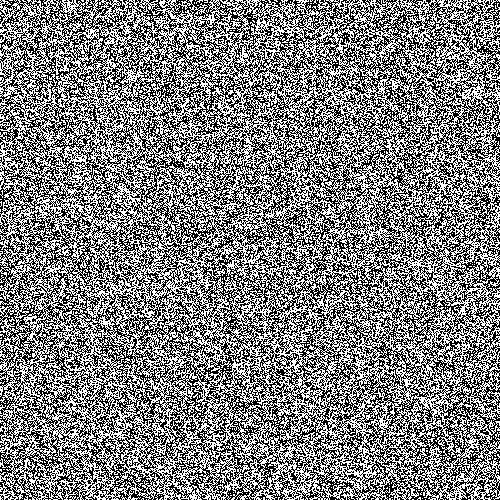
\includegraphics[width=0.75\textwidth]{rys.13.przykladowa-mikrostruktura.jpg}
    \caption{Przykładowe zdjęcie mikrostruktury. Przedstawia ono instancję ze zbioru $R_m$, gdzie zdjęcia są pogrupowane ze względu na wytrzymałość na rozciąganie. W tym przypadku jest to mikrostruktura o małej odporności. Żródło: \cite{Pirowski17}}
    \label{fig:mesh13}
\end{figure}
W prawym dolnym rogu każdego ujęcia znajduje się skala zaznaczona na czerwono, która pokazuje rzeczywistą odległość określonego fragmentu ze zdjęcia. Czarne struktury na szarym tle to powracający motyw na tych fotografiach. Są to składniki strukturalne stopów żelazo-węgiel, które dzielimy na sześć głównych kategorii na podstawie ich kształtu. Klasy te przedstawiono na rysunku \ref{fig:mesh14}. Będą one wykorzystywane jako dane wejściowe (tj. liczba struktur każdej z kategorii) dla tradycyjnych modeli kategoryzacji w badaniach. Oznacza to, że podobnie jak specjalici w tej dziedzinie, spróbujemy prognozować właściwości mechaniczne odlewów na podstawie liczby różnych form w mikrostrukturach. Porównanie wiedzy specjalistycznej z wiedzą wydobytą przez klasyfikatory będzie proste, dzięki czemu modele będą wysoce interpretowalne. Na końcu będziemożna porównać te wyniki z wynikami sieci neuronowej. W tym celu zostanie wykorzystane biblioteka \textit{numpy}, aby załadować i przechowywać dane. Klasyfikatory zostały zaimportowane z pakietu \textit{scikit-learn}, który dostarcza wszystkie wymagane przez nas metody. 
\begin{figure}[h]
    \centering
    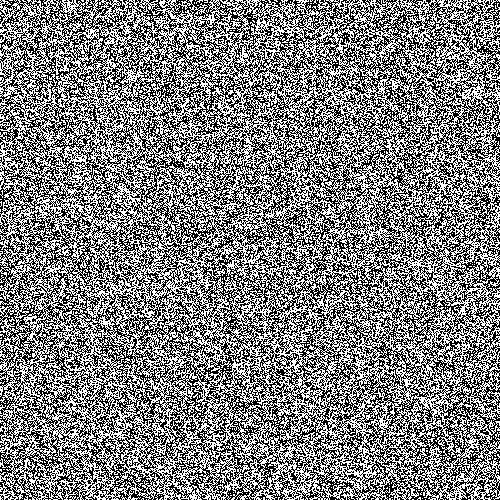
\includegraphics[width=0.62\textwidth]{rys.14.obrazy.referencyjne.png}
    \caption{Obrazy referencyjne dla głównych form grafitowych w żeliwie. Żródło: \cite{norma}}
    \label{fig:mesh14}
\end{figure}
Ponieważ dane w postaci kształtów nie są dostępne, wytworzenie takich danych, jak również infrastruktury do ich wyodrębniania, musiało być wykonane oddzielnie, co szczegółowo opisano w rozdziale \ref{sec:przygotowanie_danych}.

% ########### Przygotowanie danych ###############
\section{Przygotowanie danych}
\label{sec:przygotowanie_danych}

Postępując zgodnie z metodologią CRISP-DM, kolejnym etapem jest przygotowanie danych, które składa się z następujących podetapów:
\begin{itemize}
\item czyszczenie danych – między innymi usunięcie zdjęć, które zbytnio odstawały od reszty instancji (bądź też były zaszumione, nie zawierały informacji umożliwiających ich zidentyfikowanie),
\item wykonanie przekształceń – normalizacja danych, sprowadzenie zdjęć do tych samych rozmiarów (rozdzielczości), a także tej samej skali.
\end{itemize}
Postępując zgodnie z podaną kolejnością, na samym początku usunięto wszystkie zdjęcia najsłabszej jakości oraz te, które nie były wykonane techniką LOM, bądź też reprezentowały odlewy innego typu. Przykładowa taka instancja jest przedstawiona na rysunku \ref{fig:mesh15}. % TODO: ponizej jest napisane, ze uzywam skali. Zastanowic sie, czy to zostawic czy usunac
\begin{figure}[h]
    \centering
    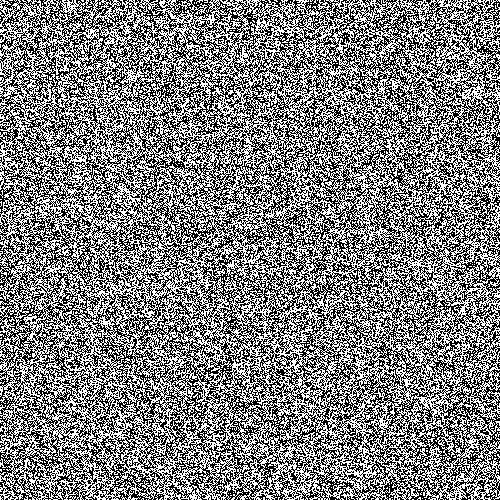
\includegraphics[width=0.62\textwidth]{rys.15.przykladowe-usuniete.jpg}
    \caption{Jeden z kilku odrzuconych obrazów. Porównując go z rysunkiem \ref{fig:mesh13} widzimy, że wielką trudnoć sprawiłoby wyodrębnienie czarnych struktur (patrz rys. \ref{fig:mesh14}). Żródło: \cite{Pirowski17}}
    \label{fig:mesh15}
\end{figure}
Natomiast druga faza, a więc normalizacja danych, jest procesem znacznie bardziej istotnym i trudniejszym. Praca nad tym aspektem projektu trwała wiele dni i została podzielona na kilka etapów:
\begin{enumerate}
\item normalizacja przybliżenia – jak wcześniej wspomniano, fotografie miały różne przybliżenia, dlatego pierwszym krokiem było ich sprowadzenie do tego samego przybliżenia. Zdecydowano, że najlepszą opcją jest powiększenie wszystkich zdjęć do przybliżenia 500x, co ma kilka zalet, w tym prostotę i rozszerzenie zbioru danych.
\item normalizacja skali – mimo że obrazy były w przybliżeniu podobne, zdarzało się, że długość podziałki dla jednego obrazu różniła się od długości podziałki dla innego obrazu.
\end{enumerate}
Poniższe sekcje zawierają wyjaśnienie tych etapów.


% ########### Normalizacja przybliżenia ###############
\subsection{Normalizacja przybliżenia}
\label{sec:normalizacja_przyblizenia}

W tym kroku wszystkie zdjęcia zostały wczytane, a następnie wszystkie fotografie o przybliżeniu różnym niż 500 razy zostały pocięte na mniejsze. Obrazy o powiększeniu 500x są zachowywane, natomiast obrazy w powiększeniu około 100x są dzielone na 25 mniejszych części i zapisywane w nowej bazie danych (rys. \ref{fig:mesh16}). Ponadto rozmiar bramki dla zdjęć wynosił 335 x 251 (szerokość x  wysokość). Po tej fazie uzyskaliśmy 2400 fotografii z początkowej liczby 115 zdjęć mikrostruktur dla podstawy Rp oraz 4757 zdjęć z początkowej liczby 223 zdjęć mikrostruktur dla podstawy Rm. Podsumowując, statystyki dla obu baz danych po tej fazie są następujące:
\begin{outline}
	\1 Rm (wytrzymałość na rozciąganie):
		\2 liczba zdjęć reprezentujących niską wytrzymałość wzrosła z 65 do 1397,
		\2 liczba zdjęć reprezentujących wysoką wytrzymałość wzrosła ze 158 do 3400,
		\2 łączna liczba zdjęć wzrosła z 223 do 4757,
		\2 24 zdjęcia miały przybliżenie 500x, 199 zdjęć miało przybliżenie 100x;
	\1 Rp (granica sprężystości):
		\2 liczba zdjęć w tym przypadku również średnio wzrosła aż dwudziestokrotnie
\end{outline}
Dodatkowo w trakcie badania wyeliminowano zdjęcia ze znaczną ilością czerwonego odcienia (czyli takie, na których skala mocno zniekształca obraz).
\begin{figure}[h]
    \centering
    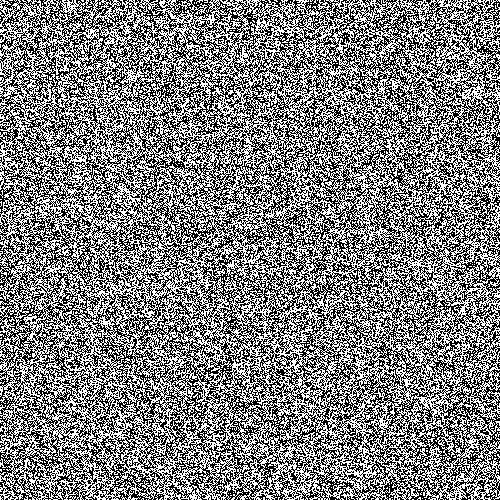
\includegraphics[width=1\textwidth]{rys.16.schemat.rozcinania.png}
    \caption{Schemat rozcinania obrazków o przybliżeniu 100x na 25 mniejszych fragmentów. Żródło: opracowanie własne z użyciem danych z \cite{Pirowski17}}
    \label{fig:mesh16}
\end{figure}
Udało się to osiągnąć, wykonując analizę histograficzną kanału czerwonego w zakresie 220-256 i usuwając zdjęcia z ponad 3000 pikseli w tym przedziale. W rezultacie liczba obrazków została nieznacznie zredukowana. Manipulacja zdjęciami była możliwa między innymi dzięki bibliotece \textit{PIL}.


% ########### Normalizacja skali ###############
\subsection{Normalizacja skali}
\label{sec:normalizacja_skali}

Jak już wspomniano wczeniej, zdarzało się, iż mimo tego samego przybliżenia, dwa zdjęcia nieznacznie różniły się pod względem skali. Można to było zauważyć na skali, która znajduje się na każdej fotografii w prawym dolnym rogu. Mimo, iż zdjęcia miały to samo przybliżenie, to ta sama odległość na dwóch różnych zdjęciach mogła odpowiadać innej długości w rzeczywistoci. Dlatego zdecydowano, aby znormalizować te dane również pod tym względem. Rozwiązanie zostało zaczerpnięte z pracy \cite{Reczek21}, która operowała na tym samym zestawie danych, a polegało ono na redukcji wszystkich kolorów oprócz tego, którego użyto do oznaczenia podziałki. Następnie, za pomocą operacji morfologicznych wykrywano poziomą linię, dzięki czemu można było wyznaznaczyć jej końce, a tym samym obliczyć jej długość. Na rys. \ref{fig:mesh17} przedstawiono wizualny wynik tych operacji. Wynik liczbowy natomiast był zapisywany w nazwie pliku. 
\begin{figure}[h]
    \centering
    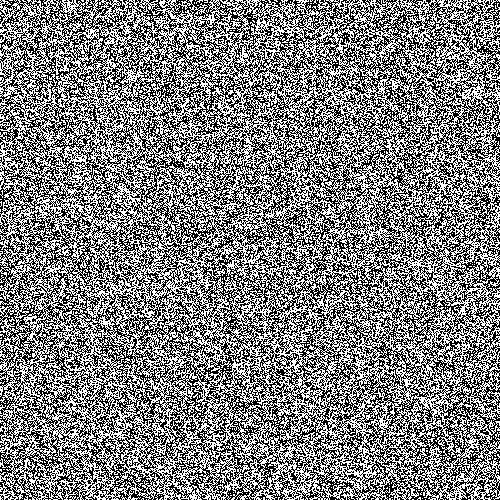
\includegraphics[width=0.5\textwidth]{rys.17.podzialka.skali.png}
    \caption{Przykładowy obrazek z poprawnie wykrytą na nim podziałką skali. Żródło: opracowanie własne przy wykorzystaniu \cite{Reczek21, Pirowski17}}
    \label{fig:mesh17}
\end{figure}
Dzięki takiej wizualnej reprezentacji można było zweryfikować poprawność w ten sposób wyznaczonej długości podziałki. Ze względu na to, iż tekst reprezentujący rzeczywistą długość podziałki był w tym samym kolorze zdarzały się błędy, jak na rysunku \ref{fig:mesh18}. 
\begin{figure}[h]
    \centering
    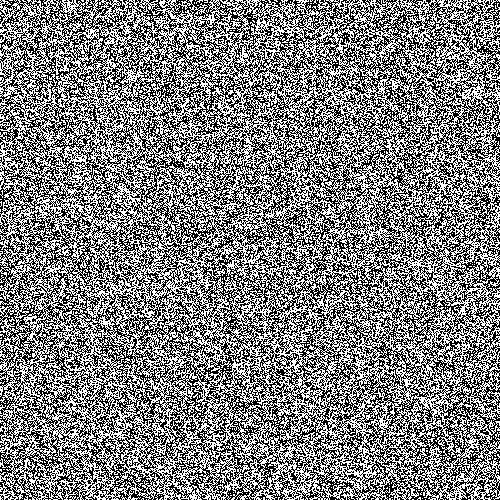
\includegraphics[width=0.3\textwidth]{rys.18.podzialka.skali.niepoprawnie.png}
    \caption{Przykładowy obrazek z niepoprawnie wykrytą na nim podziałką skali. Żródło: opracowanie własne przy wykorzystaniu \cite{Reczek21, Pirowski17}}
    \label{fig:mesh18}
\end{figure}
Aczkolwiek po przeanalizowaniu wyników okazuje się, że skuteczność tej metody wynosi aż 99\%, a więc bez problemu można ją wykorzystać w dalszych badaniach.

% ########### Augmentacja ###############
\section{Augmentacja}
\label{sec:augmentacja}

Augmentacja, a więc rozszerzenie danych to techniki służące do zwiększenia iloci danych poprzez modyfikację kopii istniejących danych (patrz \ref{cha:cha3.4}). Proces ten teoretycznie można podpiąć pod poprzedni punikt, czyli przygotowanie danych, a w szczególności, wykonanie przekształceń. Jednakże jest to obszerny temat, który zawiera w sobie wiele różnych podejść, dlatego powięcono mu cały osobny podrozdział. 

W badaniach wykorzystano kilka rodzajów augmentacji. Najpierw zastosowano technikę zwaną przycinaniem (ang. \ita{cropping}). Polegała ona na pocięciu obrazów o przybliżeniu 100x na 25 mniejszych części. Proces ten został szczegółowo opisany w rozdziale \ref{sec:normalizacja_przyblizenia}. Kolejnym zastosowanym podejściem jest skalowanie (ang. \ita{scaling}).  Polega ono na zeskalowaniu obrazów tak, aby odcinki tej samej długości na obrazku odpowiadały tej samej długości w rzeczywistości. Proces ten jest szczegółowo opisany w rozdziale \ref{sec:normalizacja_skali}. Następną techniką wykorzystaną w badaniach było odbicie (ang. \ita{flipping}).
\begin{figure}[h]
    \centering
    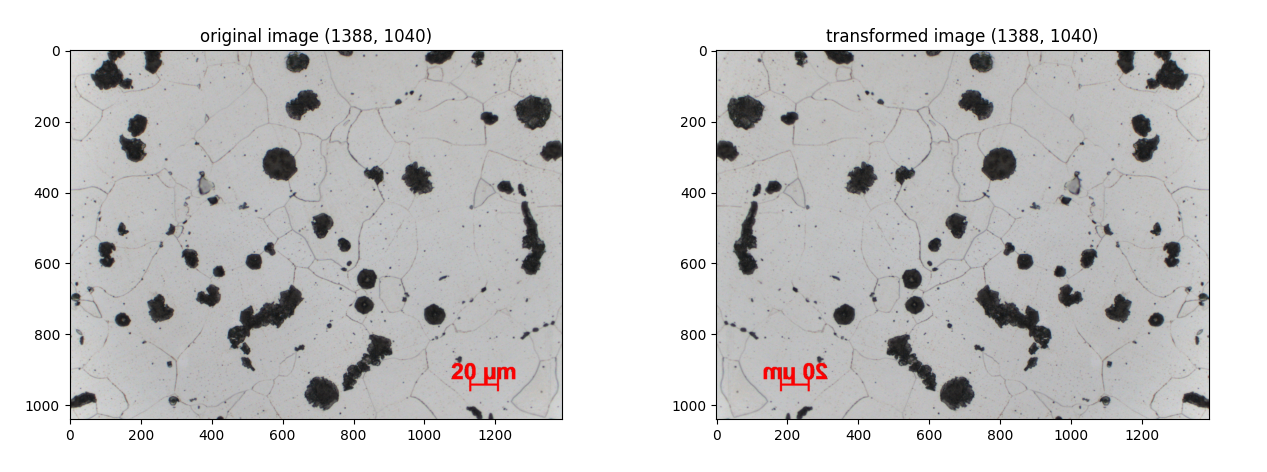
\includegraphics[width=1\textwidth]{rys.19.flipped.horizontally2.png}
    \caption{Wynik zastosowania techniki odbicia na przykładowym zdjęciu (po prawej). Widzimy, że rozmiary zdjęcia się nie zmieniają. Dodatkowo, analogicznie otrzymujemy Żródło: opracowanie własne z użyciem danych z \cite{Pirowski17}}
    \label{fig:mesh19}
\end{figure}
Dzięki tej technice możliwe jest nawet czterokrotne powiększenie zestawu danych! Dodatkową, bardzo dużą zaletą tej metody jest fakt, że nie zmienia ona wymiarów obrazów. Jest to szczególnie korzystne, ponieważ posiadane  dane nie mają tej samej szerokości i długości, co uniemożliwia wykorzystanie technik modyfikujących wymiary. Ze względu na dużą nierównowagę klas metoda ta jest wykorzystywana głównie do kompensowania liczności klas rzadkich. Przykład odbicia horyzontelnego został przedstawiony na rysunku \ref{fig:mesh19}.















